\documentclass[conference]{IEEEtran}
\IEEEoverridecommandlockouts
% The preceding line is only needed to identify funding in the first footnote. If that is unneeded, please comment it out.
\usepackage{tikz}
\usetikzlibrary{arrows.meta}
\usepackage{pgfplots}
\pgfplotsset{compat=1.18}
\usepackage{cite}
\usepackage{amsmath,amssymb,amsfonts}
\usepackage{algorithmic}
\usepackage{graphicx}
\usepackage{textcomp}
\usepackage{xcolor}
\usepackage{hyperref}
\usepackage{url}
\usepackage{enumitem}
\def\BibTeX{{\rm B\kern-.05em{\sc i\kern-.025em b}\kern-.08em
    T\kern-.1667em\lower.7ex\hbox{E}\kern-.125emX}}

% \hypersetup{
%   hidelinks,
%   pdfauthor={},
%   pdftitle={},
%   pdfsubject={},
%   pdfkeywords={}
% }

\begin{document}

\title{Monero: a privacy-focused cryptocurrency}

\author{
\IEEEauthorblockN{Andrea Altomare}
\IEEEauthorblockA{
2199451\\
\textit{Cybersecurity}\\
\textit{Department of Computer Science}\\
\textit{Faculty of Information Engineering, Computer Science and Statistics}\\
\textit{Sapienza University of Rome}\\
Rome, Italy\\
altomare.2199451@studenti.uniroma1.it
}
% \and
% \IEEEauthorblockN{Coauthor Name Surname}
% \IEEEauthorblockA{
% Affiliation\\
% City, Country\\
% email@example.com
% }
}

\maketitle

\begin{abstract}
In this document, the technology powering the Monero cryptocurrency is analyzed. Monero is a cryptocurrency that aims at solving pitfalls related to privacy and anonymity raised by Bitcoin and other common blockchains. Monero elegantly solves problem like unlinkability, untraceability, amount hiding and double spending by a heavy use of cryptographic primitives based on the Elliptic Curve. Moreover, other technologies and methods are used to further make the analysis of the Monero blockchain unfeasible by an external observer, thus making it a paramount tool for online privacy regarding economical transactions in the modern digital landscape.\\
A background on the blockchain technology is given to provide basic understanding of its functions and how it is relevant for the specific case of Monero.
\end{abstract}

\begin{IEEEkeywords}
Blockchains, cryptocurrency, cryptography, Monero, privacy
\end{IEEEkeywords}


% =========================
% 1. Introduction
% =========================
\section{Introduction}
In recent years, blockchain technology has rapidly established itself as the foundation for cryptocurrencies, digital economic assets that aim to serve as an alternative means of exchange to traditional (fiat) currencies~\cite{blockchain_adoption}. This technology, combined with modern means of communication (the Internet), allows economic transactions between individuals without the need for third-party entities to exercise authority over the medium. The properties of distributed systems are used to reach an agreement among all participants in the network and thus establish the validity of a transaction. Various techniques are also used to manage the issuance of currency and several other aspects that enable the proper functioning of the network of participants and the blockchain.\\
Examples of cryptocurrencies that have experienced significant growth in trading volumes and therefore in market value include, to name a few, Bitcoin, Ether, XRP (Ripple), and Solana~\cite{coin_market_cap}. Although similar in their fundamental functioning, each blockchain has certain peculiarities that make it more or less suitable for certain uses.\\

In its infancy and still today, Bitcoin is one of the most widely used cryptocurrency for online transactions~\cite{coin_market_cap} as an alternative to traditional means such as credit or debit cards. Due to its decentralized nature and its use as an alternative medium of exchange, Bitcoin was particularly well-suited to resist censorship by national authorities. However, as its use increased, fundamental problems emerged that Bitcoin was unable to solve, posing serious challenges to its use as an alternative to traditional currencies. Bitcoin transactions are traceable, the anonymity provided is only pseudo-anonymity, the amounts of currency exchanged can be clearly verified by anyone~\cite{bitcoin_auditable}. Bitcoin is therefore a transparent blockchain and thus unsuitable in the case of authorities who actually want to censor the medium of exchange or investigate its users.\\

Monero is a cryptocurrency designed to solve the problems raised by the use of transparent blockchains like Bitcoin. It offers:
\begin{itemize}
    \item privacy by default;
    \item fungible coins;
    \item better decentralization;
    \item transactions opaque to external observers;
    \item untraceability and unlinkability.
\end{itemize}
Monero's features are made possible thanks to the way transactions are designed, through the extensive use of Elliptic Curve Cryptography, and other core design principles whose mathematical foundations allow for the privacy and anonymity objectives necessary for a cryptocurrency truly resistant to censorship and third-party control.


% =========================
% 2. Background
% =========================

\section{Background}
\subsection{Motivations}
With the advent of information technology and the use of software for civilian purposes, one of the many sectors revolutionized by its use is the management of monetary and financial resources. Monetary transactions can be made between individuals and companies, public entities, or other individuals through the internet. The technology supporting this is based on a model in which users rely on a third-party entity (a payment institution) to validate financial transactions, track them, and safeguard their resources. This type of system is called \textbf{centralized} because control is exerted by a single central authority to verify and manage the resources and financial exchanges between the parties (the users).\\
This model, while effective for many use cases, suffers from some significant disadvantages. The entity responsible for managing the system has the authority to prevent users from using resources should any arbitrary reason exist. Furthermore, having full control of the resources, the entity effectively constitutes a \textit{single point of failure (SPOF)}: controlling the entity (for example, through laws, policies, or even cyberattacks) can effectively disrupt the proper functioning of the entire system. For all these reasons, users wishing to use the system must place trust in the authority of the designated entity.

\subsection{Historical background}
One solution to the problem of centralizing responsibility for system management is to distribute the system itself among its users, who then become active participants. This shifts from a centralized model to a distributed one. Communication between the various parties involved is made possible, as in the case of the centralized model, by traditional communication systems such as the Internet.\\
\begin{quote}
Blockchains are tamper evident and tamper resistant digital ledgers implemented in a distributed fashion (i.e., without a central repository) and usually without a central authority (i.e., a bank, company or government). At their basic level, they enable a community of users to record transactions in a shared ledger within that community, such that under normal operation of the blockchain network no transaction can be changed once published~\cite{blockchain_nist_definition}.
\end{quote}
So a \textbf{blockchain} can be viewed as a distributed data structure whose nodes (i.e., the system participants) contribute to its management and maintenance through a particular consensus protocol. Economic assets that rely on a blockchain to function are called \textit{cryptocurrencies}. A more precise definition of \textbf{cryptocurrency} is given by the American NIST (National Institute of Standards and Technology):
\begin{quote}
A digital asset/credit/unit within the system, which is cryptographically sent from one blockchain network user to another. In the case of cryptocurrency creation (such as the reward for mining), the publishing node includes a transaction sending the newly created cryptocurrency to one or more blockchain network users~\cite{blockchain_nist_definition}.
\end{quote}
The Bitcoin blockchain is the first and most famous successful example of a blockchain used as a distributed ledger for economic transactions. It was designed by Satoshi Nakamoto (a pseudonym for an unidentified individual or group of individuals), who published the idea in 2008 in the paper ``Bitcoin: A Peer-to-Peer Electronic Cash System''~\cite{bitcoin_paper}.

\subsection{Technical Background}
The following discussion of blockchain-related concepts is based primarily on the work of Narayanan \emph{et al.}: \emph{Bitcoin and Cryptocurrency Technologies: A Comprehensive Introduction}~\cite{bitcoin_narayanan}.
\subsubsection{Transactions}
In a blockchain, transactions are recorded in contiguous blocks. Each user has a pair of keys: a public key and a private key. The public key is used to generate a public address that identifies a recipient, while the private key is used to cryptographically sign transactions. A \textit{wallet} is a software used to store and manage these keys and for making new transactions.\\
The content of a block is used to calculate a hash, which is then inserted into the next block. This allows for verification of any tampering with the data in a block, since changing the data also changes the block's hash, and thus the error propagates throughout the chain, invalidating all subsequent transactions. Thanks to the calculation of hashes and the use of cryptography, the \textbf{integrity} and \textbf{unforgeability} properties of the transactions recorded in the ledger can be guaranteed. The nodes (users) that calculate hashes are called \textit{miners}. For calculating hashes and thus creating new blocks, they are incentivized by \textit{fees} included in each transaction and by a reward system whereby they are rewarded with the issuance of new cryptocurrency.\\
Transactions can be broadcast by any user on the network and will then be included in a block after verification of their correctness. A transaction can group together multiple inputs (incoming transactions) and have multiple destination outputs. Fees are the result of the difference between inputs and outputs. The relationship that must be verified is $\sum_i \text{Input}_i = \sum_j \text{Output}_j + \text{Fee}$. The output of a transaction cannot be spent twice, and different blockchains have different methods for verifying it. This model is known as \textit{UTXO (Unspent Transaction Output)} from the Bitcoin jargon.

\subsubsection{Consensus}
The state of the system is decided based on a \textbf{consensus protocol} that establishes the rules by which a new block can be valid and part of the canonical chain. The blockchain is usually a public and \textit{permissionless} system, meaning there is no third-party authority authorizing new users to join the system's network~\cite{permissionless_blockchains}. Such a distributed system can suffer from \textit{Byzantine gegeneral problem}: system participants could behave arbitrarily in a malicious manner, undermining its integrity~\cite{byzantine_systems}. A system is said to be \textbf{Byzantine fault tolerant (BFT)} if it is capable of tolerating the presence of \textit{byzantine} users, i.e., users with arbitrary behavior, within it. If the number of users in the system is not known \textit{a priori} (as is usually the case with blockchains), BFT can only be achieved probabilistically~\cite{permissionless_bft}. To achieve a system resilient to Byzantine actors, blockchains can use \textbf{Proof of Work (PoW)} consensus protocols that guarantee a block hash computation time long enough to make tampering with the blockchain economically unprofitable~\cite{pow_for_bft}. In particular, each miner does not compute a simple hash for a block, but must compute a hash whose numerical value is less than a certain target value. In this way, hash calculation becomes a sort of cryptographic puzzle to be solved, and the expenditure of computational resources makes it economically unviable to waste time calculating hashes of counterfeit blocks and thus attack the integrity of the chain. The term \textbf{hashrate} indicates the rate at which hashes are computed by miners in a PoW blockchain, measured in hashes per second (H/s): it quantifies the computational power devoted to solving the cryptographic puzzle required to add a block to the chain. Higher network hashrate generally indicates greater security and resistance to attacks~\cite{hashrate}. Complete control of the chain (that is, rewriting the history of the chain by crafting arbitrary blocks) would require more than 50\% of the total computing power of the network~\cite{attack_51}, which is therefore impractical given the current level of blockchain technology adoption.\\
The activity of mining new blocks of a blockchain is usually organized under a collective effort to solve as quick as possible the cryptographic puzzles by sharing computing power. Organizations that offer this possibility are named \textbf{mining pools} and are often very important to let new adopters of a cryptocurrency contribute to the mining process without it being economically inconvenient.~\cite{mining_pools}

\subsubsection{Longest chain rule}
If multiple miners manage to simultaneously create different new blocks, the state of the chain may become inconsistent, resulting in \textit{forks}: different branches of the same chain. In these cases, the branch that needed the most cumulative work to be mined will become part of the \textit{canonical} chain, telling what is considered to be the true state of the system. This mechanism is called \textit{longest chain rule} because tipically the branch with most cumulative work required to be mined corresponds to the longest one.~\cite{longest_chain}\\
\textbf{Finality} refers to the period of time required to be sufficiently certain that transactions included into a block will not be reverted or changed~\cite{finality_meaning}.

\subsection{Heterogeneity of different blockchains}
It is important to note that different blockchains may adopt different rules and operations depending on their intended use case and the efficiency and scalability objectives for which they were designed. However, the operation described above reflects a sufficiently general approach that is also useful for understanding the Monero blockchain.


% =========================
% 3. History & Governance
% =========================

\section{History \& Governance}
\subsection{History}
The spread of Bitcoin as a medium of exchange on the internet paved the way for its use as a preferred medium of exchange in environments requiring higher levels of privacy than those guaranteed by traditional means such as credit cards and bank accounts. Specifically, Bitcoin allows for pseudo-anonymity through the use of public addresses not directly linked to an individual. As Bitcoin's popularity grew, private \textbf{central exchanges} emerged, allowing purchases of the cryptocurrency using fiat currency. As Bitcoin became increasingly common as a currency for commerce and trading, national authorities in several countries required exchanges to implement measures aimed at knowing their customers (KYC, \textit{Know Your Customer}) and combating money laundering (AML, \textit{Anti-Money Laundering}). These measures were necessary because Bitcoin and other cryptocurrencies could be used as a means for tax evasion or avoidance, as well as for illegal activities~\cite{crypto_money_laundering}. With these security measures in place, a person's identity could be linked to their public address, and since transactions were publicly recorded on the blockchain, their online activity could be tracked~\cite{bitcoin_auditable}. This highlighted the problems posed by Bitcoin and other common cryptocurrencies: anonymity was ineffective, and tighter control by authorities effectively restricted the use of cryptocurrencies. However, this was not only a problem for criminals, but also for ordinary individuals concerned about their online privacy and who used the medium solely to avoid censorship by a central authority, regardless of the reason.\\
In 2012, \textbf{CryptoNote} was published: a \textit{white paper} that outlined the design of a protocol that addressed the problems posed by Bitcoin~\cite{cryptonote}. CryptoNote was the foundation upon which \textbf{Bytecoin} was born in 2012~\cite{bytecoin}, the first attempt to implement this protocol. However, Bytecoin was subject of concern from the online community, particularly regarding the cryptocurrency pre-mining, which would have allowed blockchain developers to gain an unfair advantage~\cite{mastering_monero}.\\
In 2014, a fork of Bytecoin gave rise to \textbf{Bitmonero}, an implementation of the CryptoNote protocol that finally resolved the ethical concerns raised by Bytecoin~\cite{mastering_monero}. Following the hard fork, the project was eventually renamed simply \textbf{Monero} (which translates to \textit{coin} in Esperanto), and the online community involved in the fork from Bytecoin took over the leadership~\cite{monero_brief_history}. The code used to identify the monetary currency of the Monero blockchain across markets and block explorers is \textit{XMR}~\cite{coinmarketcap_monero}.

\subsection{Governance}
Monero does not have a formal governance system based on voting tokens or an administration that exercises unquestionable authority. Rather, it relies on the cooperation of multiple workgroups that drive the development and evolution of its blockchain~\cite{monero_workgroups}.
\subsubsection{Core Team}
The Core Team is a group of individuals who manage Monero's critical infrastructure. Its responsibilities are administrative and custodial. Specifically, it manages access to the development repository (on the online platform GitHub~\cite{monero_repo}), controls contributions to the Monero software codebase, and approves merges after review.\\
The Core Team is also responsible for the project's financial management through the \textit{Community Crowdfunding System (CCS)}.
It is also responsible for managing the infrastructure associated with Monero, which makes it publicly accessible, such as the website (\href{https://www.getmonero.org}{getmonero.org}) and its domain.\\
The Core Team can act as a mediator in the event of deadlocks regarding the development of new blockchain features.

\subsubsection{Monero Research Lab}
The Research Lab (MRL) is a workgroup composed of cryptography researchers who are working on the evolution of the Monero protocol in its critical cryptographic aspects, which enable it to achieve the privacy and anonymity standards required by the nature of the project. The MRL produces formal, peer-reviewed papers that analyze new cryptographic schemes and model threat vectors.\\
MRL ensures the feasibility of the Monero community's proposals and their security standards, so that new features do not compromise the security and mathematical integrity of the system's privacy model.

\subsubsection{Other workgroups}
There are several workgroups, each dealing with different aspects of Monero's development as an ``ecosystem''. Some of the most relevant are:
\begin{itemize}
    \item Development workgroups: These workgroups develop the CLI and GUI for wallets and the Monero daemon;
    \item Community workgroup: A workgroup used by the community for organization and coordination;
    \item Localization workgroup: This workgroup is responsible for translating Monero-related software and documentation.
\end{itemize}
A comprehensive list of workgroups and their functions is provided in the ``Workgroups'' section of the official website.~\cite{monero_workgroups}

\subsubsection{Community Crowdfunding System}
Of particular importance is the ``Community Crowdfunding System'' (CCS), the system through which Monero's development is funded. Its operations are summarized below.
\begin{enumerate}
    \item A proposal to contribute to the Monero ecosystem is submitted via a \textit{Merge Request (MR)} to the CCS Proposal repository on GitLab~\cite{ccs_repo_gitlab}, specifying the work to be done, a timeline, and the cost in XMR.
    \item The community analyzes the proposal and discusses its pros and cons.
    \item The submitter modifies it, if necessary, in accordance with community suggestions and feedback.
    \item If a loose consensus is reached among community members, the Core Team approves the MR and funding begins.
    \item Once funding is completed (not guaranteed), the proposal goes into \textit{Work in Progress} status and the submitter begins work on it (or continues, if they have already started).
    \item The Core Team distributes funding only when development milestones are reached and verified by the community.
    \item Once all milestones are completed, the proposal is moved into \textit{Complete Proposals}.
\end{enumerate}
Full information can be found on the official website~\cite{monero_ccs}.


% =========================
% 4. Consensus Mechanism
% =========================

\section{Consensus Mechanism}
The discussions in this and the following sections are broadly based on the works of \emph{Zero to Monero: Second Edition} (by koe, Kurt M. Alonso, and Sarang Noether)~\cite{zero_to_monero_2} and \emph{Mastering Monero: The future of private transactions} (by SerHack and the Monero Community)~\cite{mastering_monero}, two of the most authoritative resources for studying and understanding Monero and its blockchain, as recommended by the official Monero website~\cite{monero_library}.

\subsection{Motivation for an ASIC-resistant protocol}
Monero is a public, permissionless blockchain. Like other blockchains, Monero achieves Byzantine fault tolerance thanks to a \textbf{Proof of Work} consensus protocol. The design of Monero's PoW protocol is based on the idea that centralizing computational resources could undermine the proper functioning of the blockchain or give an unfair advantage to individuals or groups with greater economic resources. PoW protocols are typically based on solving a ``cryptographic puzzle'' (specifically, calculating a hash): whoever manages to solve these puzzles in the shortest time receives a reward in the native currency of the blockchain on which they mine. For this reason, owning more powerful hardware than other participants in the network constitutes a financial incentive for a miner. Over the years, the computation hardware for the aforementioned cryptographic problems has transitioned from simple CPUs to GPUs, then to FPGAs (\textit{Field-Programmable Gate Arrays}), and finally to ASICs (\textit{Application-Specific Integrated Circuits})~\cite{bitcoin_asics_dominance}. ASICs are specialized hardware capable of performing the computations required to solve cryptographic puzzles faster than other hardware devices. In Bitcoin, for example, the economic incentive provided by the reward guaranteed by its PoW protocol led to the increasingly widespread adoption of ASIC devices. The fundamental problem is that computational power is therefore concentrated in the hands of a few groups of individuals who build actual \textit{mining farms} to collect the rewards for new blocks (called, in Bitcoin jargon, \textit{coinbase})~\cite{bitcoin_asics_dominance}. Concentration of computing power is a risk factor because, if a single group were to reach more than 50\% of capacity, it could, as described above, attack the integrity of the blockchain~\cite{attack_51}.\\
\textbf{RandomX} is Monero's PoW protocol~\cite{monero_technical_specs}. It was designed specifically to overcome these problems, making a scenario in which a few groups achieve a critical concentration of computing power in the network much more difficult. The underlying idea is that the cryptographic problem to be solved should not be solvable using dedicated hardware such as ASICs, so that each participant can effectively and efficiently participate in the consensus on the state of the blockchain. For this feature, the RandomX protocol is said to be \textbf{ASIC-resistant}~\cite{randomx_design}.

\subsection{Overview of the protocol}
The idea behind RandomX is that the cryptographic puzzle to be solved need not to be a ``fixed'' and knowable problem \textit{a priori}, since if it were, dedicated hardware could be built to efficiently solve that specific problem. RandomX addresses this criticality by requiring, as its name suggests, that the problem to be solved be random each time: the solution algorithm is therefore not fixed but dynamic, and changes based on the actual problem to be solved.\\
The protocol works as follows~\cite{randomx_design}:
\begin{enumerate}
    \item A random program is generated based on the data in the block to be mined;
    \item The program is translated into machine code;
    \item The program is executed;
    \item A hash is calculated on the result of the computation.
\end{enumerate}

\subsection{RandomX Virtual Machine}
The code generated from the data in the block to be mined is executed in a dedicated virtual machine. The operations performed on the VM are heterogeneous (e.g., integer operations, floating-point operations, cache accesses, RAM accesses), requiring their execution to involve multiple units of a modern CPU and memory accesses so that each generated program is as close as possible to a general-purpose problem that cannot be solved by dedicated hardware. The main elements involved in the computing environment are~\cite{randomx_design}:
\begin{itemize}
    \item 64-bit and 128-bit \textbf{registers}: these simulate the general-purpose and SIMD\footnote{\textit{Single instruction, multiple data} registers hold a vector of multiple data elements and enable parallel operations on them through SIMD instructions.} registers of a processor;
    \item \textbf{scratchpad}: a 2~MiB memory area, designed to fit in the cache of a modern CPU;
    \item \textbf{dataset}: a memory area allocated in RAM ($\sim$2~GB).
\end{itemize}

The RandomX Instruction Set Architecture (ISA) provides 64-bit instruction encoding. Each of the 8 bytes of an instruction has a specific role (e.g., opcode, source, destination). Opcodes are encoded with 8 bits, but the number of available operations is less than 256: more 8-bit values are associated with the same opcode, so that the probability of having instructions involving the ALU and FPU is greater compared to having flow control or memory access instructions. This results in execution similar to that of any general-purpose program.

\subsection{Execution of the protocol}
Before starting mining, the VM dataset is initialized using the \textit{Argon2d} hash function, taking as input the header of a \textit{key block} (a block, preceding the one to be mined, whose height is divisible by 2048)~\cite{randomx_github}.\\
Considering the mining of a new block, the RandomX execution flow is as follows~\cite{randomx_design}.
\begin{enumerate}
    \item The block header and a nonce are taken (the \textit{nonce} is a random number). A seed is calculated from this data using the \textit{BLAKE2b} cryptographic hash function.
    \item The seed is fed into a Pseudo-Random Number Generator (PRNG), which generates a sequence of 64-bit numbers. Each number represents a single 8-byte instruction. This random sequence of instructions is compiled just-in-time, providing the program that will be executed.
    \item The scratchpad is then filled with pseudo-random data derived from the previously calculated seed.
    \item The program is executed, reading and writing data to memory and changing the state of the registers according to the instructions.
    \item Once execution is complete, the final state of the VM (given by registers and scratchpad) is hashed using the BLAKE2b hash function.
    \item The resulting hash value is compared to the network target: if it is less than the target, the block is solved and can be added to the chain.
    \item If the hash value is greater than the target, the execution is repeated, incrementing the nonce.
\end{enumerate}
An in-depth assessment of the RandomX algorithm is presented in Quarkslab’s ``RandomX - Security Audit''~\cite{randomx_quarkslab}.


% =========================
% 5. Privacy of the Transactions
% =========================

\section{Privacy of the Transactions}\label{sec:transactions}
A key aspect of achieving Monero's privacy goals is ensuring that transactions made on its blockchain are truly private (anonymous) and untraceable. Monero implements a privacy stack that conceals the destination, the source, and the amount of currency involved in the transaction.

% ---------- PRIVACY OF THE RECEIVER STEALTH ADDRESSES ----------

\subsection{Privacy of the receiver - Stealth addresses}
Privacy goals regarding the recipient of a transaction are achieved in two ways. The first involves the privacy of the recipient's address involved in a transaction recorded on the blockchain.\\
Monero adopts a dual-key architecture. Each user has a pair of keys, one called the \textbf{view key} and the other the \textbf{spend key}, each of which is used for a specific purpose within a transaction. Each key pair consists of a public key and a private key.

\subsubsection{View key pair}
This is the key pair used for receiving funds. Let the pair be $(a, A)$,
\begin{itemize}
\item $a$ is the \textbf{private view key}: it is used to observe incoming transactions;
\item $A$ is the \textbf{public view key}: it is part of the user's total public key.
\end{itemize}

\subsubsection{Spend key pair}
This is the key pair used to sign transactions and spend funds. Denoted as $(b, B)$,
\begin{itemize}
\item $b$ is the \textbf{private spend key}: it is used to sign a new transaction;
\item $B$ is the \textbf{public spend key}: it is part of the user's total public key.
\end{itemize}
A user's public address is given by the two public keys, therefore: $(A, B)$.\\

Recipient privacy is achieved through the use of \textbf{stealth addresses}. Given \textit{Alice} and \textit{Bob} as two network users, if Alice wants to send XMR to Bob, she won't do so using her public address but will instead obtain a one-time address for that specific transaction. This way, if an outside observer wanted to determine who Alice sent the funds to, they wouldn't be able to connect that address to Bob's identity. This unique address is the stealth address.\\

Monero uses elliptic curve cryptography as the cryptographic system for transactions in its blockchain. The calculations used to obtain stealth addresses are based on the twisted Edwards curve \textbf{Edwards25519}~\cite{monero_ed25519} (additional technical details are provided in Appendix~\ref{app:ecc_overview}).\\
The procedure for obtaining a stealth address is as follows~\cite{cryptonote, zero_to_monero_2}.
\begin{enumerate}
\item The recipient's public address $(A, B)$ is taken.
\item A \textbf{transaction private key} $r$ is generated: a 256-bit integer modulo l ($l \approx 2^{252}$).
\item A shared secret $rA$ is computed (the secrets are exchanged via a non-interactive ECDH, Elliptic-curve Diffie–Hellman exchange).
\item The stealth address is created using the formula:
\[
P = H_s(r \cdot A) \cdot G + B
\]
$H_s$ is the hash function \textit{Keccak-256}, $G$ is a base point of the elliptic curve.
\item The transaction is created with the tuple $(P, R)$, where $P$ is the computed stealth address and $R = rG$ is known as the \textit{transaction public key} \cite{zero_to_monero_2} and allows the ECDH exchange. Note that $P$ cannot be traced back to either $A$ or $B$ without knowing their respective private keys, so it is not possible to connect the stealth address $P$ to its real recipient.
\end{enumerate}
The transaction is then recorded in a block of the chain.\\

The recipient's wallet \textit{Bob} constantly scans every single new transaction in the blockchain, looking for those intended for him. For each transaction, the scanning process is as follows~\cite{zero_to_monero_2}:
\begin{enumerate}
\item He takes the transaction public key $R$.
\item He calculates the shared secret using his private view key: $aR$ (Note: $aR = rA$, see Appendix~\ref{app:ecdh}).
\item Compute the stealth address associated with the shared secret:
\[
P' = H_s(a \cdot R) \cdot G + B
\]
\item If $P' = P$, where $P$ is the stealth address of the analyzed transaction, Bob is indeed the recipient of the transaction.
\end{enumerate}

Once Bob has determined that a transaction is addressed to him, he can proceed to spend his funds using his private spend key. To use the funds as input for a new transaction, he must first \textit{unlock} the transaction by mathematically reconstructing the private key associated with the transaction he was the recipient of. In the context of elliptic curve cryptography, this means finding the integer $k$ such that: $kG = P$ ($P$ is the stealth address of the transaction to be unlocked).\\
The procedure is as follows~\cite{zero_to_monero_2}:
\begin{enumerate}
\item Bob computes the hash of the shared secret:
\[
x = H_s(aR)
\]
\item Bob knows that his public spend key $B$ was used to construct the stealth address, and in elliptic curve cryptography the relationship $B = bG$ holds.
\item Putting the two elements together, we have:
\[
P = H_s(aR) + B = xG + bG
\]
\item Therefore:
\[
P = (x + b)G \implies k = x + b \implies k = H_s(aR) + b
\]
\item Having the private transaction key $k$, Bob can spend the funds by signing a new transaction and using the unlocked \textit{outputs}.
\end{enumerate}

% ---------- PRIVACY OF THE RECEIVER SUBADDRESSES ----------

\subsection{Privacy of the receiver - Subaddresses}
The privacy of the recipient of a transaction is also achieved through the use of fictitious addresses called \textit{subaddresses}, which serve to protect a user even outside the context of the Monero blockchain~\cite{mastering_monero}.\\
A \textbf{subaddress} is a secondary address derived from a user's public address~\cite{zero_to_monero_2, mastering_monero}. The need for subaddresses arises when a user wants to use their public address to receive funds on the Monero blockchain, publishing the address in contexts such as websites, social networks, or through any other non-private means of communication. The scenario in which fictitious addresses become necessary is when two individuals collude to discover the identity of a target user. For example:
\begin{enumerate}
\item Bob and Alice know each other personally. Bob provides Alice with his public address to pay for a service or product he sold her.
\item Bob also uses the same public address to purchase XMR in exchange for another cryptocurrency, such as Bitcoin, on a centralized exchange.
\item An investigation is opened against Bob, suspected of selling illegal goods.
\item Authorities trace Alice, one of Bob's buyers, and discover that Alice makes payments to a certain public address.
\item Authorities interrogate several centralized exchanges in search of transactions involving the obtained Monero public address.
\item Bob's central exchange responds positively to the authorities' request, and through its KYC\footnote{\textit{Know Your Customer}: a policy requiring an exchange or service provider to know the legal identity of its customers.} policy, it is able to uniquely link the Monero public address to Bob's legal identity.
\item Bob's identity is therefore revealed.
\end{enumerate}
If Bob had used a subaddress, the scenario described above would have been impossible: by giving two different subaddresses to Alice and the exchange, it would have been impossible to link them to his identity.\\
It's worth noting that in the case described above, Alice would also have gotten into trouble with the authorities for purchasing illegal goods. Therefore, it's also in the best interest of anyone sending funds to a Monero user to use a subaddress instead of the standard public address whenever possible. The two types of addresses can be distinguished because they are identified by a leading byte, called \textit{network byte}~\cite{mastering_monero}, which indicates their version: a standard address begins with \texttt{4}~\cite{mastering_monero}, while a subaddress begins with \texttt{8}~\cite{mastering_monero}.\\

Subaddresses allow you to deterministically generate a large number of addresses from a single wallet seed.\\
A subaddress is defined by a pair of indices $(i, j)$, where $i$ is the account index and $j$ is the subaddress index. The wallet calculates a subaddress-specific scalar $m$, starting from the private view key $a$ and the indices:
\[
m = H_s(a \ || \ i \ | | \ j)
\]
The wallet then generates the \textbf{subaddress public spend key} ($D$):
\[
D = B + m \cdot G
\]
Finally, the wallet generates the \textbf{subaddress public view key} ($C$):
\[
C = a \cdot D
\]
The complete subaddress is therefore the pair $(C, D)$.~\cite{subaddresses_doc, subaddresses_mrl}\\

Transaction construction differs when a subaddress is involved~\cite{subaddresses_doc, subaddresses_mrl}.
\begin{enumerate}
\item The transaction public key is computed using the public spend key $D$ instead of the elliptic curve base point $G$:
\[
R = r \cdot D
\]
\item The shared secret is computed:
\[
S_{shared} = r \cdot C
\]
\item The stealth address is then computed as:
\[
P = H_s(r \cdot C) \cdot G + D
\]
\end{enumerate}
\medskip
The recipient's wallet (e.g., Bob) ``listens'' for incoming transactions: it scans incoming blocks and performs the following flow of operations~\cite{subaddresses_doc, subaddresses_mrl}.
\begin{enumerate}
\item Compute the shared secret:
\[
S'_{shared} = a \cdot R
\]
Note that if the transaction is addressed to Bob, $S' = S$. Indeed:
\[
a \cdot R = a(rD) = r(aD) = r \cdot C \implies S' = S
\]
Formal justifications for the above equalities are provided in Appendix~\ref{app:ecdh}.
\item The wallet must now determine whether the transaction's stealth address belongs to it. In particular, it must compute the public spend key $D_{candidate}$ that satisfies the equation:
\[
D_{candidate} = P - H_s(a \cdot R) \cdot G
\]
\item Bob's wallet finally checks whether $D_{candidate}$ exists in its pre-computed table of subaddress spend keys. If it finds a match, the wallet recognizes that the transaction is intended for it, and identifies exactly which subaddress received it by using the indices $(i, j)$.
\end{enumerate}

% ---------- AMOUNT HIDING RINGCT ----------

\subsection{Amount hiding - RingCT}
An important aspect of transaction privacy involves hiding the amount of cryptocurrency involved in a transaction. This is not only important from a purely privacy perspective, but also mitigates attack vectors aimed at deanonymizing a user, not strictly related to the functioning of the blockchain but rather to social aspects of economic management (for example, analyzing spending patterns or large amounts transfers).\\
Monero uses the protocol called \textbf{RingCT} (\textit{Ring Confidential
Transactions})~\cite{ringct, zero_to_monero_2} to obfuscate the amount of cryptocurrency involved in a transaction. RingCT incorporates two specific technologies for quantity hiding, and integrates them with ring signatures to hide the sender of a transaction (see: \autoref{subsec:ring_signatures}).\\

\subsubsection{Pedersen Commitments}
When sending XMR on the Monero blockchain, it should be impossible for any external observer not involved in the transaction to know the amount sent. However, it should be possible to verify that the amount spent does not exceed the sender's available cryptocurrency. This is made possible by \textbf{Pedersen commitments}~\cite{pedersen_commitments}, a cryptographic mechanism that allows a number (the amount of cryptocurrency) to be cryptographically hidden while still allowing algebraic verification as if it were applied to the clear text amount.\\
A public commitment $C$ is calculated as~\cite{ringct, zero_to_monero_2}:
\[
C = xG + aH
\]
where:
\begin{itemize}
\item $G$ and $H$ are two base points of the elliptic curve;
\item $x$ is a random blinding factor; using the ECDH of this factor, the recipient will be able to decrypt the commitment and know the amount of funds received;
\item $a$ is the amount of cryptocurrency involved.
\end{itemize}
In each transaction, the \textit{Inputs} (that are previously received transaction outputs) must be sufficient to cover the entire cost, including the \textit{Outputs} (the amount to be sent to the recipient) and the \textit{fee} (the payment guaranteed to miners for including the transaction in a block)~\cite{zero_to_monero_2}. Miners, not being directly involved in the transaction, cannot know the input and output quantities, since they are hidden by a commitment, but they must still be able to verify their correctness. Pedersen commitments have the property of \textbf{additive homomorphism}: the sum of the commitments is equal to the commitment of the sum~\cite{zero_to_monero_2}. The mathematical verification is possible as follows~\cite{zero_to_monero_2}.\\
Let
\begin{align*}
C_{in} &= x_{in}G + a_{in}H \\
C_{out} &= x_{out}G + a_{out}H \\
C_{fee} &= x_{fee}G + a_{fee}H
\end{align*}
be the calculated commitments. With simple algebraic steps, we have:
\[
C_{in} - C_{out} - C_{fee} = (x_{in} - x_{out} - x_{fee})G + (a_{in} - a_{out} - a_{fee})H
\]
If $a_{in} = a_{out} + a_{fee}$ then the term with $H$ vanishes. Therefore:
\[
C_{in} - C_{out} - C_{fee} = (x_{in} - x_{out} - x_{fee})G
\]
Hence:
\[
\sum_{i} C_{in, i} - \left( \sum_{j} C_{out, j} + C_{fee} \right) = 0 \cdot H + k \cdot G
\]
where $k$ is the difference between the blinding factors. Specifically, the blinding factors are random numbers chosen so that their sum (between input and output) is equal to 0~\cite{zero_to_monero_2, pedersen_commitments_relations_detail}. Thus:
\[
\sum_{i} C_{in, i} - \left( \sum_{j} C_{out, j} + C_{fee} \right) = 0
\]

A miner can know the value of the fee and be incentivized to include the transaction in a block because the fee is inserted in the clear text within the transaction data~\cite{zero_to_monero_2}, and the fee commitment is calculated as:
\[
C_{fee} = (0 \cdot G) + (fee \cdot H)
\]
The commitment is therefore calculated without the blinding factor~\cite{zero_to_monero_2}, and the miner, in addition to verifying the correctness of the transaction as explained above, can verify that the fee declared in the clear text by the sender is the one used to calculate $C_{fee}$, and is therefore valid.

\subsubsection{Bulletproofs+}
Pedersen commitments are based on modular arithmetic. Each quantity $a \in \mathbb{Z}_l$, that is, $a$ is an element of the group of integers $\mathbb{Z}$ modulo $l$~\cite{pedersen_commitments} ($l \approx 2^{252}$~\cite{monero_ed25519}). Pedersen commitments have a flaw when working with negative numbers, precisely because of modular arithmetic. In particular, it is possible to use multiples of the modulo $l$ to create cryptocurrency \emph{ex nihilo}~\cite{zero_to_monero_2}.\\
In modular arithmetic we have:
\[
l - 1 \equiv -1 \pmod{l}
\]
A malicious user could therefore construct a transaction such that:
\begin{itemize}
\item input: $10$ XMR;
\item output 1: $100$ XMR;
\item output 2: ($l - 90$) XMR ($\equiv -90$).
\end{itemize}
The relationship between input and output then becomes:
\[
Input = Output_1 + Output_2 \implies 10 = 100 - 90
\]
which is a valid relationship for a miner (who cannot know that one of the values is negative). Therefore, by using only $10$ XMR as input and sending $-90$ XMR to a secondary address (for example, to one subaddress of their own), the malicious user is effectively able to arbitrarily ``create'' $90$ XMR ($100 - 10$ XMR) and send it to another user, perhaps for purchasing a good.\\
The problem just described could lead to what is known as \textbf{hidden inflation issue}\footnote{Hidden inflation is an undetected increase in the effective money supply (e.g., unauthorized or unaccounted issuance) that dilutes existing holders' purchasing power.}, and the solution employed by Monero is implemented by the zero-knowledge \textbf{Bulletproofs+}~\cite{bulletproofs_plus} protocol. Each commitment must come with a \textbf{range proof} that proves that the value of XMR falls within a range, specifically $[0, 2^{64} - 1]$~\cite{zero_to_monero_2}, by calculating a \textbf{Weighted Inner Product} argument~\cite{bulletproofs_plus, bulletproofs_plus_security_audit}.

% ---------- PRIVACY OF THE SENDER RING SIGNATURES ----------

\subsection{Privacy of the sender \& untraceability - Ring Signatures}\label{subsec:ring_signatures}
The final critical piece for achieving full privacy within a transaction is the privacy of the sender and the \textbf{untraceability} of the transactions. This is important for two main reasons. First, it is useful for a user not to be linked to their online activity or the users who interact with them, so it is necessary to make it impossible for an outside observer to understand \textit{where} the funds received come from. On the other hand, it may also be useful for the sender not to be known to the recipient of their transactions. Second, the \textbf{fungibility} of a currency requires that each unit of the currency in question be spendable in the same way as every other. In blockchains like Bitcoin, every transaction is traceable back to its initial source~\cite{bitcoin_auditable}. If funds originating from a transaction are known, at any point in their history, to have been involved in transactions resulting from fraudulent or malicious activity, or otherwise in violation of the law or policy of a regulatory authority, the use of those funds can be rendered illegitimate by censoring the outputs from which those funds originate, effectively rendering the currency implemented by the blockchain non-fully fungible.\\
Monero uses ring signatures to make transactions untraceable and hide their sender~\cite{cryptonote, zero_to_monero_2}. A \textbf{ring signature} is a cryptographic scheme which makes it possible to specify a set of possible signers without revealing which member actually produced the signature~\cite{ring_signature}. Specifically, the sender signs a transaction using a set of public keys $\{P_1, P_2, \dots, P_n\}$ that includes his or her public key $P_{\pi}$, so that anyone verifying the transaction's legitimacy can verify that \textit{someone} actually signed the transaction, but cannot determine exactly \textit{who}~\cite{ringct}. The cryptographic scheme used by Monero is called \textbf{CLSAG \textit{(Concise Linkable Spontaneous Anonymous Group)}}~\cite{zero_to_monero_2, clsag}. A CLSAG signature proves that the signer knows the private spend key $x$ and the private amount blinding factor $z$ corresponding to a certain index $\pi$, without revealing $\pi$~\cite{ringct, zero_to_monero_2}.\\
Let the ring $R$ consist of $n$ pairs of public keys (unspent output keys) and corresponding Pedersen commitments~\cite{ringct}:
\[
R = \{ (P_1, C_1), (P_2, C_2), \dots, (P_n, C_n) \}
\]
The true signer holds the secret index $\pi$, the private spend key $x$ (where $P_{\pi} = xG$), and the blinding factor $z$ (where $C_{\pi} = aH + zG$). The signer also computes the Key Image $I = xH_p(P_{\pi})$, which is the unique identifier of the spent funds (further discussion on Key Images later in this section).\\
The protocol for the sender to create a transaction is summarized below~\cite{cryptonote, zero_to_monero_2}.
\begin{enumerate}
\item The sender (e.g., Alice) identifies the output they wish to spend.
\item The sender's wallet scans the blockchain and selects 15 additional outputs (called \textbf{decoys}) using a specific statistical distribution.
\item The wallet constructs the ring signature via CLSAG, using its own output and the decoys. The signature proves that Alice owns one of the unspent outputs in the ring.
\item The wallet computes the unique Key Image and attaches it to the transaction.
\item The transaction is finally broadcast to the network.
\end{enumerate}

\medskip
The effectiveness of the ring signature mechanism also depends on how the decoys are chosen. Indeed, by choosing decoy outputs that are too old, the true output used to create the new transaction would be distinguishable from the others, leading to a possible identification of the true output used and thus deanonymization of the sender~\cite{traceability_monero_blockchain} (and fungibility issues of the output itself, as discussed previously).\\
Decoys are selected based on their age based on a \textbf{Gamma distribution}~\cite{zero_to_monero_2}. The Gamma distribution mimics real human spending behavior~\cite{gamma_sampling} and is essential for mitigating possible statistical deanonymization attacks based on the age of the outputs. No authorization is required from the true owners of the decoy outputs to use them to build the ring. In this way, when constructing a transaction, a wallet can operate without the need to communicate with external nodes, thus avoiding to open the way to other possible attack vectors.\\

A fundamental element for the correct functioning of the RingCT system is the presence of the \textbf{Key Image}~\cite{key_image}: a value associated with the output of a transaction which allows the verification that the funds have not already been spent.\\
In particular, since who needs to verify the transaction does not know the actual being spent, due to the ring signature, it could not be verified whether that output has already been spent previously. To overcome this problem, a value, the Key Image, is attached to the transaction so that, even without knowing the output being spent, it can be verified that that output has not already been spent, thus solving a potential \textbf{double-spending} problem.\\
The Key Image is calculated as~\cite{zero_to_monero_2, key_image}:
\[
I = xH_p(P)
\]
where
\begin{itemize}
\item $x$ is the one-time private spend key,
\item $P$ is the one-time public spend key ($P = xG$),
\item $H_p$ is a hash-to-point function (based on Keccak).
\end{itemize}
The transaction verifier will check the absence of the Key Image from the spent output database: if the Key Image is already present, the double-spending attempt is detected and the transaction is rejected as invalid. This is possible because the calculated value of the Key Image is deterministic: the one-time private $x$ and public $P$ spend keys will always yield the same value, thus making the keys for an output unusable after the first time they are used~\cite{zero_to_monero_2}. Note that using the private key $x$ makes it impossible for an external observer to determine the true output spent in a transaction from its Key Image, as this cannot be reconstructed solely from the public keys of the outputs in the ring.\\

Finally, it should be noted that creating a new output in a transaction may require aggregating multiple inputs into one. For example, if Alice has 1 XMR in one unspent output and 2 XMR in another, and wants to send 3 XMR to Bob, she will need to use both unspent outputs in question as inputs to send the correct amount. Alice's wallet will then create a ``multi-input transaction'' by building a ring signature for each input, separately. Each input will be checked separately for validity to validate the transaction~\cite{ringct, zero_to_monero_2, mastering_monero}.


% =========================
% 6. Protection of the Network Layer
% =========================

\section{Protection of the Network Layer}
\subsection{Protection over the Monero network}
Transaction construction mechanisms allow Monero to achieve ``on-blockchain'' privacy through the use of cryptography. These mechanisms make it impossible (or better, statistically infeasible) for an external observer to determine the source of a transaction, its recipient, and the amount of cryptocurrency involved. However, there is a class of attacks that allow the deanonymization of the source of a transaction and which rely on the functioning of the peer-to-peer network itself.~\cite{mastering_monero}\\
When a user creates a transaction, it is broadcast to neighboring nodes in the network via a simple gossip protocol. An adversary (for example, an authority interested in payment system censorship) could install several Monero nodes in the network so that one of its nodes will statistically be the first one to receive and process a new transaction broadcast from a Monero user to the network. In this way, the node that first receives the transaction is able to determine its origin by associating it with the node from which it originated (i.e., its IP address). Furthermore, communications on the Monero network are unencrypted, making it possible for a malicious actor acting as a \textit{man-in-the-middle} to eavesdrop communications between two or more network nodes.~\cite{dandelion_plus_plus}\\

The solution to this problem, which is infrastructural in nature rather than related to the blockchain itself, is achieved by Monero through the implementation of \textbf{Dandelion++}~\cite{dandelion_plus_plus}, a special transaction propagation protocol designed to disguise their true origin. Dandelion++ is an improvement on the original Dandelion protocol already proposed for Bitcoin (BIP 156)~\cite{bip_156}.\\
The protocol constructs an \textit{anonymity set}: a set of nodes that constitute a \textit{privacy subgraph}, chosen randomly and that will receive a newly created transaction before other nodes in the network. The set of nodes is kept unchanged for a period called the \textit{epoch}, which lasts approximately 10 minutes~\cite{dandelion_plus_plus}. This is essential to counteract the case where multiple nodes in the anonymity set are controlled by an adversary.\\
The phases of the propagation protocol are as follows~\cite{dandelion_plus_plus}.

\subsubsection{Stem phase (anonymity)}
\begin{enumerate}[label=(\alph*)]
\item The wallet sends the transaction to a randomly selected peer from the privacy subgraph.
\item The selected relay (i.e., node) receives the transaction and, based on a stochastic process (a biased coin flip), decides whether to remain in the stem phase or move on to the next phase. If the biased coin flip is successful ($\sim80\%$ probability), the node forwards the transaction to only one of its peers.
\item This ensures that if the next node in the privacy subgraph is a spy node, it still cannot determine whether the transaction originated from the node it came from or a previous node.
\end{enumerate}
\medskip
\subsubsection{Fluff phase (diffusion)}
\begin{enumerate}[label=(\alph*)]
\item If the biased coin flip fails ($\sim20\%$ probability), the node currently holding the transaction enters the diffusion phase. This also happens when a randomized timer expires (so as to ensure the end of the stem phase).
\item The node then floods the network with the transaction via a simple gossip protocol.
\item Nodes in the peer-to-peer network now see that the transaction originated from the node in the fluff phase, which is not the original source. The true sender of the transaction therefore remains hidden.
\end{enumerate}
\medskip

\begin{figure}%[!t]
  \centering
  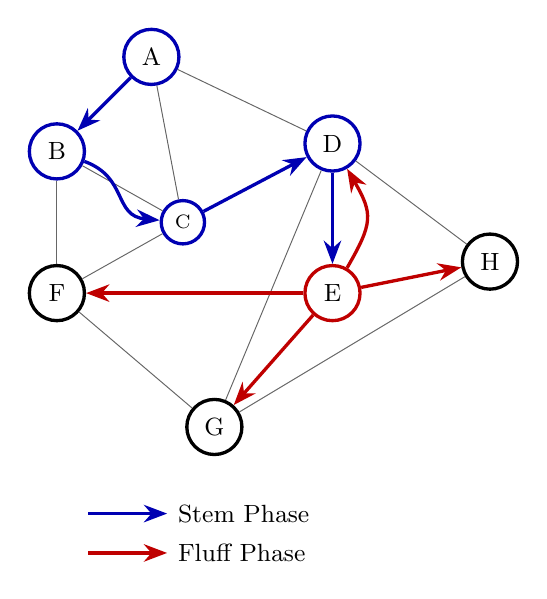
\begin{tikzpicture}[
    font=\small,
    stem/.style={->,>=Stealth,very thick,draw=blue!70!black},
    fluff/.style={->,>=Stealth,very thick,draw=red!75!black},
    net/.style={draw=black!60, line width=0.35pt},
    stemnode/.style={circle,draw=blue!70!black,very thick,minimum size=7mm,inner sep=0pt,fill=white},
    stemnodeSmall/.style={stemnode,minimum size=5.5mm,font=\scriptsize},
    fluffnode/.style={circle,draw=red!75!black,very thick,minimum size=7mm,inner sep=0pt,fill=white},
    othernode/.style={circle,draw=black,very thick,minimum size=7mm,inner sep=0pt,fill=white}
  ]

  % --- Nodes ---
  \node[stemnode]      (A) at (0.0,3.2) {A};
  \node[stemnode]      (B) at (-1.2,2.0) {B};
  \node[stemnodeSmall] (C) at (0.4,1.1) {C};
  \node[stemnode]      (D) at (2.3,2.1) {D};

  \node[fluffnode]     (E) at (2.3,0.2) {E};

  \node[othernode]     (F) at (-1.2,0.2) {F};
  \node[othernode]     (G) at (0.8,-1.5) {G};
  \node[othernode]     (H) at (4.3,0.6) {H};

  % --- Thin network links ---
  \draw[net] (A) -- (C);
  \draw[net] (A) -- (D);
  \draw[net] (B) -- (C);
  \draw[net] (B) -- (F);
  \draw[net] (C) -- (F);
  \draw[net] (F) -- (G);
  \draw[net] (G) -- (H);
  \draw[net] (D) -- (H);
  \draw[net] (D) -- (G);

  % --- Stem phase (blue) ---
  \draw[stem] (A) -- (B);
  \draw[stem] (B) to[out=-20,in=175,looseness=1.25] (C);
  \draw[stem] (C) -- (D);
  \draw[stem] (D) -- (E);

  % --- Fluff phase (red) ---
  \draw[fluff] (E) -- (F);
  \draw[fluff] (E) -- (G);
  \draw[fluff] (E) -- (H);
  \draw[fluff] (E) to[out=60,in=-60,looseness=1.35] (D);

  % --- Legend ---
  \draw[stem]  (-0.8,-2.6) -- (0.2,-2.6) node[right,black]{Stem Phase};
  \draw[fluff] (-0.8,-3.1) -- (0.2,-3.1) node[right,black]{Fluff Phase};

  \end{tikzpicture}
  \caption{Transaction propagation among nodes in Dandelion: Stem phase (blue) followed by Fluff diffusion (red).}
  \label{fig:dandelion}
\end{figure}

As shown in Fig.~\ref{fig:dandelion}, the stem phase (highlighted in blue) conveys the message through a random path and then it transitions to the fluff phase (highlighted in red) for diffusion.\\
The anonymity set is rebuilt every $\sim$10 minutes~\cite{dandelion_plus_plus} also to prevent an attacker from permanently mapping the privacy subgraph, thus degrading the protocol's privacy guarantees.\\
A potential problem during the normal flow of stem and fluff phases is a \textit{blackhole attack} implemented by a malicious node. In this type of attack, a node receiving a transaction discards it instead of forwarding it: this prevents the transaction from being verified and therefore recorded in the blockchain, causing a denial of service. To solve this problem, each node forwarding the transaction sets an \textbf{embargo timer}: if, by the end of the timer, it has not yet received the transaction back from the public network, it assumes that the stem phase has failed and therefore it broadcasts the transaction by itself~\cite{dandelion_plus_plus}.

\subsection{Protection over the Transport Layer}
Monero's P2P communication protocol operates in clear text and has no inherent cryptographic system to guarantee its \textit{confidentiality}. Monero's threat model also takes into account the case where the attacker has sufficient resources to control a large portion of the network (for example, at the ISP and autonomous system level) and is therefore able to analyze the packets exchanged between nodes, containing transactions, thus deanonymizing users. This, too, is not a flaw of the blockchain itself, but rather concerns the fundamental functioning of communication between nodes in a peer-to-peer network, which obviously occurs over the Internet.\\
To protect communication between nodes, Monero offers the ability to natively integrate with the Tor and I2P overlay networks, which provide an additional cryptographic layer to packets in transit, thus preserving the confidentiality of their contents~\cite{monero_technical_specs, monero_tor_i2p, monero_connect_wallet_tor}.\\
\textbf{Tor \textit{(The Onion Router)}} is an anonymous \textit{overlay network} based on a set of routers (called \textit{relays}) managed by volunteers. Its technology is called \textbf{Onion Routing}~\cite{tor}: data is encapsulated in several layers of packets, each encrypted with different cryptographic keys, and is routed along a random path composed of three nodes (\textit{Guard}, \textit{Middle}, \textit{Exit}). Each node decrypts only the layer needed to know the next destination, without ever being able to know the full path and therefore the origin and the final destination of the packet simultaneously, nor its contents. The relays therefore act as proxies, routing encrypted traffic and hiding the IP address of the connection's origin.~\cite{tor}\\
\textbf{I2P \textit{(Invisible Internet Project)}} is an anonymous network that operates on top of the standard internet. It is structured as a decentralized peer-to-peer network, without central directory servers (and therefore without a single point of failure). Unlike Tor, I2P uses \textbf{Garlic Routing}. This type of routing groups together multiple encrypted messages (called \textit{cloves}) directed to different recipients. Furthermore, thanks to one-way tunnels, incoming and outgoing traffic travel completely separate paths. The characteristics of the I2P network allow its users to communicate without revealing their location on the network, thus remaining anonymous.~\cite{i2p}\\

The Monero daemon (\texttt{monerod}) is designed to be network-agnostic, maintaining separate tables for peers on IPv4, IPv6, Tor, and I2P, thus decoupling communication with a node for transmitting a transaction from its IP address. Overlay networks are used primarily in the Stem Phase: the first node to receive a transaction can't even know which \textit{physical node} it came from because the source is masked behind proxies (more precisely, an \textit{exit node} in the case of Tor).\\
To start \texttt{monerod} on Tor, it needs to be used the \texttt{--tx-proxy} flag~\cite{monerod}: this allows transactions to be sent over the Tor network. It is also possible to configure a node to be reachable only via Tor by starting it as an \textit{Onion Service} using the \texttt{--anonymous-inbound} flag~\cite{monerod, advantages_of_tor_monerod}.


% =========================
% 7. Economic model
% =========================

\section{Economic Model}
Unlike other popular cryptocurrencies like Bitcoin, which have a fixed-supply and therefore deflationary economic model~\cite{bitcoin_deflationary}, Monero does not impose a hard fixed supply cap. The supply continues to grow indefinitely at a very slow rate as shown in Fig.~\ref{fig:supply_btc_xmr}, reconstructing a disinflationary dynamic, with a positive inflation rate that decreases over time. Monero's design immediately took into account the problem posed by a rigid supply cap and a limited block size, which could lead to the creation of a ``fee market'' once the total supply was reached, creating system stability problems. Monero implements an economic system governed by three main mechanisms: tail emission to solve the hard supply cap problem, dynamic block size, and dynamic fee adjustment based on network traffic over a given period to maintain market equilibrium.

\subsection{Monetary policy}
A cryptocurrency's monetary policy dictates the frequency with which new units of the currency are minted and released into the system. The issuance of new currency serves two main purposes: to distribute currency to early adopters (initial distribution) and to incentivize miners to participate correctly in verifying new blocks in order to receive a reward.\\
The original CryptoNote protocol~\cite{cryptonote}, on which Monero is based, defined the \textbf{base reward} as~\cite{monero_note_on_fees}:
\[
BaseReward = 2 \cdot \frac{M - A}{2^{20}} \cdot 10^{-12}
\]
In this equation~\cite{monero_note_on_fees}:
\begin{itemize}
\item $M$ represents the total number of atomic units available in the initial phase, defined as $2^{64} - 1$;
\item $A$ represents the current number of atomic units already generated (circulating supply);
\item $10^{-12}$ is the factor needed to divide XMR into atomic units of 12 decimal places (\textit{piconero}~\cite{monero_denominations}).
\end{itemize}
\medskip
The formula resulted in a smooth and granular reduction in the reward for each mined block. The ``smooth emission'' curve ensured a gradual and virtually imperceptible change in economic conditions from one block to the next for miners, promoting hashrate stability and allowing miners to predict and adjust operational expenditures (\textit{OpEx}) with high precision.\\
After an initial ``bootstrapping'' phase aimed at launching the Monero economic system and building the mining infrastructure by the users, the \textbf{Tail emission} phase began in June 2022~\cite{tail_emission_moneropedia}. As the reward approached \textbf{0.6 XMR} per block~\cite{monero_technical_specs}, the protocol rule dictated that the reward should not fall below that threshold. Since the beginning of the tail emission phase, the reward for each new Monero block has been 0.6 XMR. A new block is mined approximately every 2 minutes~\cite{monero_technical_specs}, so $\sim432$ XMR are emitted every day. Thanks to tail emission, there is a small but constant increase in XMR in circulation. This causes Monero's inflation rate to decrease linearly but never to reach 0\%.\\
The fixed emission of XMR allows miners to have a ``security budget'' and to counteract some problems arising from the lack of issuance of new currency. Without a reward, the incentive to mine blocks would solely be the fees associated with a transaction. This, however, would create problems for two main reasons.
\begin{itemize}
\item \textbf{Fee volatility:} During periods of low network usage, transaction fees may decrease to the point that it becomes less economically profitable to mine a block, thus leading to a decrease in hashrate and consequently making the blockchain more vulnerable to computational power-based attacks~\cite{attack_51}.
\item \textbf{Chain reorganization:} If fees are the only reward for miners, if a miner discovers a block with unusually high fees, they may be incentivized not to continue extending the chain but rather to remine that specific block to collect the fees. This leads to chain reorganizations, increasing its instability and degrading Monero's reliability as a payment network~\cite{fee_sniping}.
\end{itemize}

\begin{figure}[!t]
  \centering
  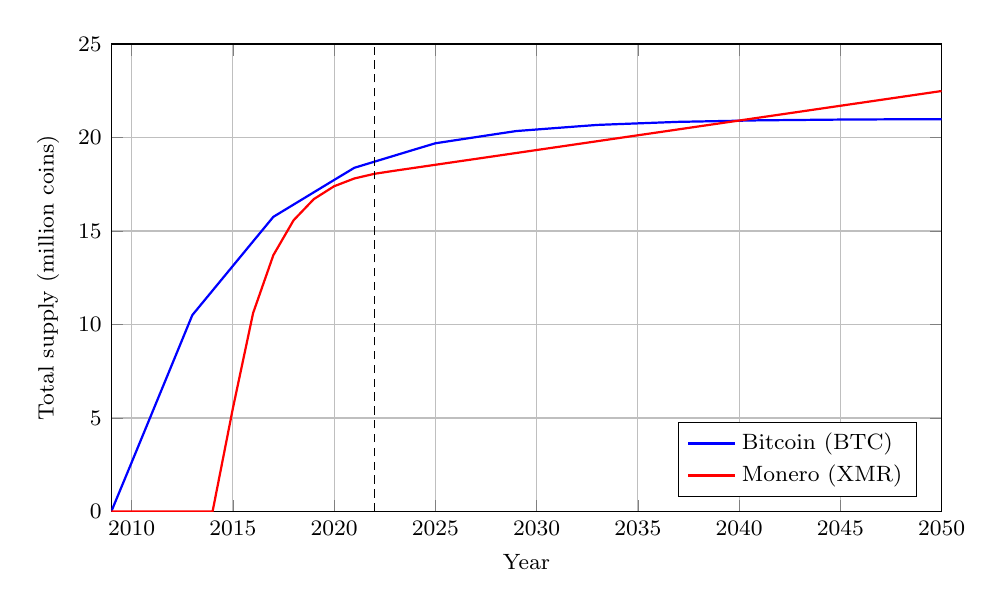
\begin{tikzpicture}
    \begin{axis}[
      xticklabel style={/pgf/number format/1000 sep={}},
      width=\columnwidth,
      height=0.62\columnwidth,
      xlabel={Year},
      ylabel={Total supply (million coins)},
      xmin=2009, xmax=2050,
      ymin=0, ymax=25,
      grid=both,
      legend pos=south east,
      legend cell align=left,
      tick label style={font=\footnotesize},
      label style={font=\footnotesize},
      legend style={font=\footnotesize},
    ]

      % --- Bitcoin (modeled, ideal 10-min blocks and 210k-block halvings) ---
      \addplot+[mark=none, thick] coordinates {
        (2009,0.0) (2010,2.614) (2011,5.242) (2012,7.87) (2013,10.502) (2014,11.816)
        (2015,13.13) (2016,14.444) (2017,15.756) (2018,16.413) (2019,17.07) (2020,17.727)
        (2021,18.38) (2022,18.709) (2023,19.037) (2024,19.366) (2025,19.691) (2026,19.856)
        (2027,20.02) (2028,20.184) (2029,20.346) (2030,20.428) (2031,20.511) (2032,20.593)
        (2033,20.673) (2034,20.715) (2035,20.756) (2036,20.797) (2037,20.837) (2038,20.857)
        (2039,20.878) (2040,20.898) (2041,20.919) (2042,20.929) (2043,20.939) (2044,20.949)
        (2045,20.959) (2046,20.964) (2047,20.97) (2048,20.975) (2049,20.98) (2050,20.982)
      };
      \addlegendentry{Bitcoin (BTC)}

      % --- Monero (modeled, 2-min blocks, tail emission 0.6 XMR/block from end-May 2022) ---
      \addplot+[mark=none, thick] coordinates {
        (2009,0.0) (2010,0.0) (2011,0.0) (2012,0.0) (2013,0.0) (2014,0.0)
        (2015,5.503) (2016,10.606) (2017,13.704) (2018,15.573) (2019,16.706) (2020,17.392)
        (2021,17.809) (2022,18.06) (2023,18.225) (2024,18.383) (2025,18.541) (2026,18.699)
        (2027,18.856) (2028,19.014) (2029,19.172) (2030,19.33) (2031,19.487) (2032,19.645)
        (2033,19.803) (2034,19.961) (2035,20.119) (2036,20.276) (2037,20.434) (2038,20.592)
        (2039,20.75) (2040,20.907) (2041,21.066) (2042,21.223) (2043,21.381) (2044,21.539)
        (2045,21.697) (2046,21.854) (2047,22.012) (2048,22.17) (2049,22.328) (2050,22.486)
      };
      \addlegendentry{Monero (XMR)}

      % Start of tail emission (end of May 2022 ~ year 2022)
      \draw[densely dashed] (axis cs:2022,0) -- (axis cs:2022,25);
      \node[anchor=south east,font=\footnotesize] at (axis cs:2022,25) {Tail emission (June 2022)};

    \end{axis}
  \end{tikzpicture}
  \caption{Total supply estimation of Bitcoin and Monero modeled under their respective issuance schedules (ideal target block intervals). Data source: moneroinflation.com~\cite{moneroinflation}.}
  \label{fig:supply_btc_xmr}
\end{figure}

\subsection{Dynamic block size and fee adjustment}
In Monero, there is no fixed block size: the size can be dynamically adjusted based on traffic (demand). If transaction volume is high, a miner can include a greater number of transactions in a block, increasing its size. This allows for increased system throughput during periods of peak demand, while maintaining efficiency.~\cite{zero_to_monero_2}\\
To prevent adversarial actors from attacking the network by overloading it with blocks that are too large, a penalty is calculated based on the size of a newly mined block and previous blocks~\cite{zero_to_monero_2}. Specifically, the network bases the calculation of the new block size limit ($M$) by looking at the median size of the last 100 blocks ($M_{100}$) and imposing a minimum threshold of 300~kB (to accommodate for periods of extremely low demand)~\cite{zero_to_monero_2}:
\[
M = \max(M_{100}, 300\text{kB})
\]
Each miner can create blocks with size $S$ such that: $S \leq 2M$. When $S \leq M$, the miner is guaranteed the full base reward (0.6 XMR). When $M < S \leq 2M$, a penalty $P$ is subtracted from the base reward $R$ for the block according to the formula:
\[
P = R \cdot \left( \frac{S}{M} - 1 \right)^2
\]
Therefore, the resulting reward becomes:
\[
R_{new} = R - P = R \cdot \left( 1 - \left( \frac{S}{M} - 1 \right)^2 \right)
\]
Finally, when $S > 2M$, the newly mined block is simply rejected for exceeding the size limit.~\cite{zero_to_monero_2}\\
Due to the reduction in the block reward, miners will increase the size of the new block only if the fees collected from the extra transactions are greater than the penalty applied to the base reward. This mechanism results in a self-regulating market: in periods of low demand, blocks are smaller and fees are lower, while in periods of higher traffic, fees must naturally increase to incentivize miners to include transactions in new blocks. In the long run, demand will tend to stabilize, so even with significant levels of high (or low) traffic, since the block size threshold $M$ varies following the last 100 blocks of the chain, the penalty will tend to 0 again and the reward guaranteed by new blocks will tend to return to the base reward of 0.6 XMR. This creates an ``economy of scale'' similar to industrial production: bandwidth becomes cheaper per unit the more it is used.~\cite{zero_to_monero_2}


% =========================
% 8. Tools & Ecosystem
% =========================

\section{Tools \& Ecosystem}
\subsection{Monero daemon (monerod)}
At the foundation of the Monero network lies the daemon, \textbf{monerod}. It acts as the backbone of the peer-to-peer (P2P) network, maintaining consensus, validating the blockchain state, and providing the necessary data API for wallets and applications.\\
\texttt{monerod} is a console-based executable written in C++ that manages the blockchain data structure. The daemon performs three primary critical functions~\cite{monerod}.
\begin{enumerate}
\item \textbf{P2P network synchronization:} It connects to other nodes to download and validate the blockchain history. This involves a heavy initial block download (IBD) phase where cryptographic proofs for every transaction in history are verified.
\item \textbf{Block validation:} It enforces consensus rules, verifying RingCT proofs, key images (to prevent double-spending), and block headers. This validation engine is the source of truth for the network.
\item \textbf{RPC API provision:} It exposes a JSON-RPC interface that allows external applications (wallets, block explorers, mining pools) to query network statistics, submit transactions, and retrieve block templates.
\end{enumerate}

\subsection{Official client implementations}
While \texttt{monerod} maintains the ledger, the official wallet software handles the cryptographic mechanisms required to interact with it. The Monero Project maintains two primary reference clients: \textbf{monero-wallet-cli} and \textbf{monero-wallet-gui}.
\subsubsection{The Command Line Interface}
The \texttt{monero-wallet-cli} is the reference implementation for wallet logic. It operates as a console application, accepting text commands to manage accounts, keys, and transactions~\cite{monero_wallet_cli}.
\subsubsection{The Graphical User Interface}
The \texttt{monero-wallet-gui} wraps the logic of the CLI/RPC into a visual application built with the Qt framework. It is designed to offer a more user-friendly experience without compromising on the underlying security model~\cite{monero_wallet_gui}.

\subsection{Wallet RPC service}
In addition to the CLI and GUI clients, Monero offers a RPC service through the \textbf{monero-wallet-rpc} HTTP server~\cite{monero_wallet_rpc}.\\
For developers building applications on top of Monero (e.g., exchanges, payment gateways, custodial services), interacting with a CLI is inefficient and error-prone. The HTTP server \texttt{monero-wallet-rpc} wraps the wallet logic into a stateless (or stateful, depending on configuration) JSON-RPC API~\cite{monero_wallet_rpc_api}.\\
Some of the use cases for Wallet RPC are the following.
\begin{itemize}
\item \textbf{Programmatic Payments:} An e-commerce backend can trigger \texttt{transfer} or \texttt{transfer\_split} calls to pay vendors automatically based on database events.~\cite{monero_wallet_rpc_api}
\item \textbf{Subaddress Management:} It allows generating thousands of unique subaddresses (\texttt{create\_address}) to distinguish customer deposits. This is vital for exchanges, which assign a unique subaddress to every user to track deposits without needing separate wallets.~\cite{monero_wallet_rpc_api}
\item \textbf{Account Partitioning:} It supports the ``Accounts'' feature, enabling a single wallet to segregate funds into logical buckets (e.g., ``Savings'', ``Operations'', ``Tax''). The RPC can query balances per account or per subaddress index.~\cite{accepting_monero}
\end{itemize}
\medskip
The strict separation between \texttt{monerod} (network data) and \texttt{monero-wallet-rpc} (private key operations) is very important for keeping the Monero’s tooling stack secure. A compromised \texttt{monerod} does not compromise keys, and a compromised wallet machine does not necessarily compromise the network node.

\subsection{Wallets classification}
Wallets in the Monero ecosystem are generally categorized by how they handle synchronization, which involves a direct trade-off between privacy, speed, and convenience. The requirement to scan every transaction on the blockchain to find those belonging to the user dictates their architecture and user experience.
\begin{itemize}
\item \textbf{Full Node Wallets:} These wallets download and verify the entire blockchain, they do not trust any external peer. They provide maximum privacy (no data leakage to remote peers) and highest censorship resistance. The cons of having a full node wallet are related to the storage capacity, bandwidth requirements, and slow initial sync. Example of this type of wallet are Monero CLI and Monero GUI (Advanced Mode).~\cite{monero_wallets}
\item \textbf{Light Wallets (Remote Node):} The wallet connects to a remote \texttt{monerod} (provided by the wallet developer, a community member, or the user's own VPS). The wallet sends its ``view key'' to the device, scans blocks locally on the phone/laptop, and identifies transactions. While this type of wallet lets its users to get fast setup with low storage requirements, it comes with some drawbacks: the remote node knows the user's IP address (unless Tor is used) and knows when the user is syncing, potentially degrading the user's anonymity. This is a ``privacy-preserving'' light client model~\cite{connect_gui_wallet_to_remote_node}. Example of this kind of wallet are Cake Wallet, Monerujo, and Feather.~\cite{monero_wallets}
\item \textbf{Light Wallet Server (LWS) clients:} These wallets offload the scanning process entirely to a server running \texttt{monero-lws}~\cite{monero_lws}, an implementation of the Monero light-wallet REST API~\cite{monero_lightwallet_api}. The user submits their private view key to the server, the server scans the chain on behalf of the user and returns a list of transactions. This mechanism lets the user achieve instant synchronization while having low power consumption (fundamental on mobile). The downsides are that the server must possess the user's view key, meaning that the server operator can see all the incoming transactions (though they cannot spend the funds). This model requires trusting the server operator with metadata. Example of this type of wallet are MyMonero and Edge.~\cite{monero_truenas}
\end{itemize}


% =========================
% 9. Regulatory Issues & Ethical Considerations
% =========================

\section{Regulatory Issues \& Ethical Considerations}
As its diffusion, popularity, and level of adoption have grown, Monero, like any payment instrument, has faced the need for regulation by national authorities~\cite{monero_illegal}. Like any cryptocurrency, Monero can be used to purchase goods or be paid for their sale, as well as a store of value and a tool for financial speculation. These aspects have made all cryptocurrencies a primary target of regulatory policies in many nation states, since without regulation they could be used for activities that are illegal, such as tax evasion, money laundering, and the purchase of illegal goods. Unlike many other cryptocurrencies, such as Bitcoin, Monero's situation is more critical from a legal perspective. Indeed, to enforce a policy on the proper use of a medium of exchange, such as a cryptocurrency, a certain degree of transparency is required, so that the authorities can carry out checks when necessary and inspect the actual use of that medium by the people who own it. Cryptocurrencies like Bitcoin use cryptography to validate transactions, ensuring their integrity and authenticity, but remain essentially ``transparent'' to the analysis of external actors~\cite{bitcoin_auditable}. The goal with which Monero was designed is precisely to achieve a level of privacy such that an external observer should not be able to understand and track the transactions recorded on the blockchain. Thanks to the mechanisms discussed in the previous chapters (\autoref{sec:transactions}), such as Stealth Addresses, RingCT, and Ring Signatures, it is impossible for an authority to clearly verify the source and recipient of the funds in a transaction, as well as the amount of cryptocurrency exchanged. Due to its nature, Monero has faced several compliance issues with the laws of several countries around the world~\cite{monero_illegal}.\\
Another significant fact is that, thanks to its privacy features, Monero is used as a preferred medium for buying and selling on the black market in darknets\footnote{A darknet is a part of the internet reachable only with dedicated software, whose content is not indexed by common search engines. Tor and I2P are examples of darknets.} and as a payment instrument for ransomware~\cite{monero_illegal_usage, crypto_money_laundering}.\\

A key measure adopted by governments in several countries has been to require central exchanges to legally identify their customers with official documents. This is especially important because when someone wants to obtain a particular cryptocurrency he often has to go through exchanges, which, having immediate availability, allow it to be purchased in exchange for fiat currency. The practice of identifying customers through official documentation (e.g., ID cards, driver's license, bank statements) is called \textbf{KYC \textit{(Know Your Customer)}}~\cite{kyc}. Central exchanges implement KYC systems to associate a legally identified person with the public addresses of their cryptocurrency wallets and the transactions they perform with these wallets. This allows exchanges to comply with the law should authorities investigate their customers. Having a clear and direct association between wallets and individuals' physical identities allows them to determine any criminal liability if those individuals are involved in illicit activities.\\
A very common use case for cryptocurrencies, given that they are relatively new and more difficult for authorities to monitor, is money laundering~\cite{crypto_money_laundering}. The KYC practice also helps authorities enforce \textbf{AML \textit{(Anti-Money Laundering)}} laws, thus enabling them to conduct financial checks on the cryptocurrency assets of individuals investigated for such crimes.\\

Due to the inherent difficulty of analyzing the Monero blockchain, and the inability to adequately implement systems to control and verify the use of assets related to it, many exchanges eventually stopped offering XMR among the cryptocurrencies purchasable on their platforms to avoid legal issues~\cite{monero_delisting_kraken, monero_delisting_binance, monero_delisting_okx}. This practice is known as \textbf{delisting}. Some countries (e.g., China, Qatar, Algeria) have gone further, banning or severely restricting privacy-based cryptocurrencies like Monero~\cite{monero_illegal}.


% =========================
% 10. Monero vs Bitcoin - Comparative Metrics
% =========================

\section{Monero vs Bitcoin - Comparative Metrics}
In the context of cryptocurrencies, Bitcoin is currently the most popular and used one (as of February 2026)~\cite{coin_market_cap}. Monero, on the other hand, is among the most used cryptocurrencies~\cite{coin_market_cap} and arguably the most used in the darknets~\cite{monero_illegal_usage}.\\
Given their level of adoption alongside similar use cases as payment systems, it is useful to make a comparison between the two cryptocurrencies, highlighting similarities and key differences that make a cryptocurrency more suitable than another depending on the purpose.

\subsection{Design philosophy}
The fundamental divergence between Bitcoin and Monero lies in their treatment of the ledger's visibility.

\subsubsection{Bitcoin}
Bitcoin operates on the principle of ``public verifiability''. The protocol ensures trust by allowing any participant to audit the entire history of the ledger. This transparency is a deliberate design choice intended to allow decentralized verification of the total supply and the validity of every transaction without relying on a third party~\cite{monero_vs_bitcoin_oak_research}.

\subsubsection{Monero}
Monero asserts that privacy is not just a feature for concealing activity but a structural requirement for ``fungibility''. Fungibility means that one unit of currency must be functionally identical to another. In Bitcoin, ``tainted'' UTXOs (Unspent Transaction Outputs) associated with illicit activities can be blacklisted by exchanges or merchants, rendering them less valuable than ``clean'' coins. For this reason, Monero was designed with the goal of providing untraceability of its transactions and mechanisms to counter analysis of its blockchain by external observers~\cite{monero_vs_bitcoin_oak_research}.

\begin{table*}[!t]
\caption{Bitcoin vs Monero: comparison summary}
\label{tab:btc_xmr_comparison}
\centering
\footnotesize
\setlength{\tabcolsep}{4pt}
\renewcommand{\arraystretch}{1.15}
\begin{tabular}{p{0.20\textwidth} p{0.38\textwidth} p{0.38\textwidth}}
\hline
\textbf{Feature} & \textbf{Bitcoin (BTC)} & \textbf{Monero (XMR)}\\
\hline
Consensus protocol &
Proof-of-Work (based on SHA-256)~\cite{bitcoin_paper}. &
Proof-of-Work (based on RandomX)~\cite{randomx_design}. \\
\hline
Nakamoto Coefficient ($NC$), Feb.~4,~2026 &
$NC = 2$ (Foundry USA 33.6\% + AntPool 19.1\%)~\cite{btc_pools_hashrateindex}. &
$NC=2$ (SupportXMR 33.5\% + Nanopool 22.6\%)~\cite{xmr_pools_poolbay}. \\
\hline
Transaction design &
``Transparent'' UTXO model: inputs spend prior outputs; new outputs remain as UTXOs until spent. Transaction data recorded in clear on the blockchain. Source and recipient are known~\cite{bitcoin_utxo}. &
Obfuscated transactions: Stealth Addresses, RingCT, CLSAG~\cite{zero_to_monero_2}. \\
\hline
Block time (target) &
$\approx$10 minutes~\cite{btc_supply_wiki}. &
$\approx$2 minutes~\cite{monero_technical_specs}. \\
\hline
Block size / weight limit &
Max block weight 4,000,000 weight units (i.e., up to $\sim$1,000,000 vbytes)~\cite{btc_glossary}. &
Dynamic block size: median $M_N$ over last $N{=}100$ blocks. Maximum allowed block size is $2M_N$ (above the median size, reward penalties are applied). Minimum 300~kB~\cite{zero_to_monero_2}.\\
\hline
Block reward \& issuance policy &
Reward halves every 210{,}000 blocks; currently 3.125 BTC/block (since 2024-04-20)~\cite{btc_supply_wiki}. &
Smooth emission until tail emission. Rewards never drop to zero: fixed at 0.6 XMR/block (or less with block-size penalties)~\cite{monero_technical_specs}. \\
\hline
Max supply &
Capped: issuance halts with 21,000,000 BTC total~\cite{btc_supply_wiki}. &
No fixed cap: fixed emission rate with perpetual tail emission (0.6 XMR/block)~\cite{zero_to_monero_2}. \\
\hline
\end{tabular}
\end{table*}

\subsection{Consensus and mining mechanisms}
The mechanism by which the network agrees on the state of the ledger lays the foundation of its security. While both utilize a Proof-of-Work (PoW) protocol, their approaches to hardware and decentralization diverges radically.

\subsubsection{Bitcoin}
Bitcoin utilizes the SHA-256 algorithm~\cite{bitcoin_paper}. It is computationally simple, requiring only integer operations, bitwise shifts, and additions. This simplicity allowed for the rapid development of Field-Programmable Gate Arrays (FPGAs) and subsequently Application-Specific Integrated Circuits (ASICs), hardware chips designed solely to mine Bitcoin. Mining has thus become an industrial-scale operation dominated by large companies and massive data centers~\cite{bitcoin_mining_centralization}.

\subsubsection{Monero}
Monero utilizes RandomX, a PoW algorithm designed to be ASIC-resistant. RandomX achieves this by requiring the execution of random code segments and extensive access to large blocks of memory. By requiring general-purpose computing (complex instruction sets, branch prediction, and memory latency) for the mining activity, RandomX ensures that the most efficient mining hardware is a general-purpose CPU. Manufacturing a ``RandomX ASIC'' would essentially ends up being a reconstruction of a high-end CPU~\cite{monero_mining}.

\subsection{Decentralization metric - Nakamoto Coefficient}
The \textbf{Nakamoto Coefficient} refers to the minimum number of independent entities (such as validators or node operators) that need to work together to disrupt the network by taking over its control or stopping block production. The higher the Nakamoto Coefficient, the more decentralized and resilient a blockchain network is against such threats~\cite{nakamoto_coefficient}.

\subsubsection{Bitcoin}
The coefficient is typically low, around 3 to 4. This means the top 3 or 4 mining pools could theoretically collude to censor transactions or reorganize the chain. However, since pools are aggregates of individual miners who can switch pools instantly, the ``real'' coefficient is arguably higher, as pool operators are tied to their miners~\cite{bitcoin_nakamoto_coefficient}.

\subsubsection{Monero}
The Nakamoto Coefficient for Monero is similar to that of Bitcoin, given that a few mining pools control the majority of the hashrate~\cite{monero_mining_pool_stats}.

\subsection{Privacy model and transaction design}
As discussed earlier, Bitcoin and Monero have been design to deal with different privacy concerns and threat models in mind.

\subsubsection{Bitcoin}
Bitcoin uses a ``transparent'' Unspent Transaction Output (UTXO) model. A transaction consumes inputs (previous UTXOs) and creates new outputs~\cite{bitcoin_utxo}. The graph of inputs and outputs is public, if user A sends BTC to user B, the link is permanent.

\subsubsection{Monero}
By the means of features like Stealth Addresses, RingCT, and CLSAG, Monero ensures higher privacy levels than Bitcoin, making the analysis of the transactions impossible by looking just at the data recorded on its blockchain.

\subsection{Summary and other quantitative metrics}
A brief summary on the comparison between Bitcoin and Monero on the aspects discussed and on some key metrics is provided in \autoref{tab:btc_xmr_comparison}.


% =========================
% 11. Security & Risk Profile
% =========================

\section{Security \& Risk Profile}
Although Monero's implementation is strictly based on rigorous mathematical and cryptographic foundations, it is of course not immune to security risks, as any other technology.

\subsection{Key Image infinite inflation bug}
The most critical class of vulnerabilities in any cryptocurrency are those that affect the monetary supply or the ability to spend funds. One of the most important threats that Monero has faced in its history is the ``Key Image'' infinite inflation bug~\cite{key_image_bug}.\\
In May 2017, a vulnerability that affected all cryptocurrencies based on CryptoNote, including Monero, was disclosed. This bug allowed an attacker to create an infinite amount of coins undetected, effectively breaking the scarcity of the asset.\\
The vulnerability was in the verification of the key image (\autoref{subsec:ring_signatures}). The exploit relied on the properties of the Ed25519 curve. The curve is a cyclic group (Appendix~\ref{app:ecc_overview}), but the implementation of the verification logic did not enforce that the key image $I$ belonged to the correct subgroup of prime order $l$. An attacker could craft a transaction with a manipulated key image that satisfied the ``incomplete'' verification checks but did not correspond to a valid, unspent output. By exploiting this, the attacker could effectively ``double-spend'' the same output repeatedly by generating different, yet mathematically valid, key images for the same funds, effectively allowing for the generation of new coins~\cite{key_image_bug}.\\
This vulnerability was patched in Monero before it could be exploited. The patch involved adding a strict subgroup check to ensure that $lI = \mathcal{O}$ (the identity element), verifying that the point lies on the main subgroup~\cite{key_image_bug}.

\subsection{``Black Marble'' spam attack}
Attackers have attempted to actively manipulate the Monero network to degrade privacy. These attacks target the decoy pool, with implications on the effective ring size.\\
The so-called ``Black Marble'' attack, happened in March 2024, was one of the most notable~\cite{black_marble_attack}. The Monero network experienced a massive surge in transaction volume, lately called the ``Black Marble'' or ``Flood'' attack. The mechanism of the attack relies on the selection of decoys for building the Ring Signature and create a transaction (\autoref{subsec:ring_signatures}). The attackers flooded the network with millions of transactions (\textit{black marbles}), transactions of which they of course knew the private keys. When a legitimate user created a transaction, the wallet randomly selected 15 decoys from the blockchain. Due to the flood, there was a high probability that many of these decoys were ``black marbles''. Since the attackers knew they did not spend the black marbles in an analyzed transaction, they could identify the actual output being spent with significantly higher probability. For example, if the attackers controlled 10 of the 15 decoys, the effective ring size dropped from 16 to 6, with the probability of recognizing the actual output being increased to $\frac{1}{6}$ instead of $\frac{1}{16}$~\cite{black_marble_analysis}.\\
The Monero community is currently actively discussing mitigations for this kind of attacks. Two of the possible solutions are~\cite{black_marble_solutions}:
\begin{itemize}
\item making the attack economically unsustainable by increasing the fees (and thus the cost) of spam transactions;
\item replacing the Ring Signature scheme entirely with a new system in which \textit{every} output on the chain is a decoy (so, the ring size would be the size of the whole set of transaction outputs ever recorded on the blockchain). This solution is actually a prominent proposed evolution of the protocol, which goes under the name of \textbf{FCMP \textit{(Full-Chain Membership Proofs)}}~\cite{fcmp}.
\end{itemize}

\subsection{Considerations on the security profile of Monero}
As discussed, Monero presented possible security issues, which were promptly resolved or which are currently under the process of being mitigated. Some of the main security flaws involve incorrect or incomplete implementation of its strong cryptographic schemes or relay on the statistical analysis of its chain, especially when targeting its anonymity guarantees~\cite{monero_security_analysis_mrl}.\\
Monero is nevertheless one of the most secure blockchains privacy-wise, remaining one of the top choice when it comes to deal with anonymity and privacy in blockchain-based payment systems~\cite{monero_privacy_guides}.


% =========================
% 12. Related Work
% =========================

\section{Related Work}
In this section, relevant works in the field of blockchains and specifically on topics related to Monero are presented.\\
Research in areas of cryptography, network security, and blockchains in general is active and constitutes the foundation upon which some of the most promising technologies are built.

\subsection{Traceability in Monero blockchain}
In the paper ``An Empirical Analysis of Traceability in the Monero Blockchain''~\cite{traceability_monero_blockchain}, Möser \emph{et al.} analyze traceability in Monero’s earlier ring signature scheme, focusing on how decoy selection can leak the real spent output. They highlight two concrete weaknesses: a ``chain-reaction'' effect where elimination across rings can reveal the true input, and a temporal or age-distribution bias where the real input tends to be the ``newest'' member of the ring, enabling privacy leakage through heuristic guessing. In their measurements, they report that a large fraction of inputs with this kind of rings is susceptible to this inference technique, and that ``guess the newest'' can achieve high accuracy.\\

This is one of the main reasons why Monero had to evolve its ring signature scheme over time, in particular its decoy selection process, to preserve the privacy of the sender of a transaction.

\subsection{Deanonymization of transactions over Tor}
In ``Deanonymizing Transactions Originating from Monero Tor Hidden Service Nodes''~\cite{monero_tor_deanonymization}, Shi \emph{et al.} present a network-layer vulnerability in the use that Monero does of Tor, showing that under certain conditions an attacker can deanonymize transactions originating from Monero Tor hidden service nodes. The core point is that transport anonymity (Tor) does not automatically imply origin anonymity against an adversary who can correlate or otherwise exploit integration or visibility assumptions at the boundary between Monero and Tor.\\

The paper demonstrates that privacy coins like Monero still face practical deanonymization issues even when their transactions are routed through anonymity networks. Network-layer protections reduce, but do not eliminate, threats deriving from the way the underlying network infrastructure works, and that adversary capability (routing observation, node control, correlation) matters as much as protocol choice.

\subsection{Post-quantum and quantum blockchains}
One of the most important threats to blockchains and in general to any other technology that relies on cryptography is the development of quantum computing. Shor's algorithm and its variations can be used to break popular ciphers whose effectiveness is based on the hardness of the factorization of prime numbers and the Discrete Logarithm Problem (and thus ECDLP, Appendix~\ref{app:ecdh})~\cite{shor_dlp}. Breaking Elliptic Curve Cryptography primitives could effectively disrupt the blockchains which are based on them (Monero being one of them). For this reason, it is essential for these technologies to evolve so they can adopt cryptographic systems immune to the threat posed by quantum computers.\\
Yang \emph{et al.} analyze and compare two broad responses to the quantum threat, in the paper ``A Survey and Comparison of Post-Quantum and Quantum Blockchains''~\cite{quantum_blockchains}. The first are post-quantum blockchains, that replace vulnerable cryptographic primitives with quantum-resistant schemes. The second are called ``quantum blockchains'', and leverage quantum communication and quantum computation to rebuild parts of the security foundations of the blockchains.\\
Discussions on post-quantum strategies regarding Monero have been made in the past years~\cite{monero_quantum_ccs}. Quantum-resistant cryptography and quantum communications will be increasingly important for making future-proof blockchains and are especially important for cryptocurrencies whose utility lies in the way they use cryptography to provide privacy and anonymity.


% =========================
% 13. Conclusions
% =========================

\section{Conclusions}
This paper has presented a comprehensive analysis of the Monero blockchain, evaluating its architectural design, cryptographic primitives, and economic incentives. As the landscape of digital assets evolves, Monero stands out as one of the most important privacy-focused cryptocurrencies, thanks to a technically rigorous implementation of fungible digital cash.\\
While early blockchains like Bitcoin have successfully implemented decentralized consensus protocols to build censorship-resistant payment systems, their transparent ledgers introduced critical privacy weaknesses. Instead, Monero effectively addresses these downsides through a ``privacy by default'' approach. Implementation of mechanisms like Stealth Addresses for receiver privacy, Ring Signatures (CLSAG scheme) for sender obfuscation, and Pedersen commitments with Bulletproofs+ for concealing transaction amounts, ensures that transaction data remains opaque to external observers while maintaining verifiable integrity.\\
Furthermore, the implementation of the RandomX consensus protocol represents a defense against the centralization of mining power, effectively mitigating the dominance of ASICs that characterizes the Bitcoin network. Moreover, Monero's economic model refuses a fixed-supply approach: the introduction of the \textit{tail emission} guarantees a perpetual security budget for miners, while the dynamic block size algorithm ensures the adaptability of the blockchain along periods with varying transaction volumes, allowing the network to scale organically with demand.\\
However, the very features that ensure censorship resistance and fungibility also place Monero at the center of regulatory debates regarding Anti-Money Laundering (AML) compliance and concerns on its use for other illicit purposes.\\
In conclusion, Monero represents a leading actor in the development of private distributed ledger technologies. As privacy becomes an increasingly important aspect in the digital age, Monero's technical features offer an important foundation for the future of secure and private digital finance.


% =========================
% Appendices
% =========================

\appendices

\section{Elliptic Curve Cryptography in Monero}\label{app:ecc}
\subsection{General overview}\label{app:ecc_overview}
Monero uses the twisted Edwards curve \textbf{Edwards25519}~\cite{monero_ed25519}, sometimes referred to as just \textit{Ed25519}~\cite{zero_to_monero_2} (which is actually the signature scheme based on the Edwards25519 curve), which offers security and performance advantages, particularly with regard to side-channel and subgroup attacks~\cite{ed25519_security}. Stealth address derivation, as well as other privacy features offered by Monero, are based on one-way functions\footnote{A \textit{one-way function} is a function that is simple to compute, but \textit{computationally difficult} to invert. Modern cryptography is based on the concept of one-way functions.} computed on the elliptic curve, so that the result of a calculation cannot be traced back to its input data.\\
Monero's cryptography is based on the finite field $\mathbb{F}_q$, and uses the curve~\cite{cryptonote}:
\[
-x^2 + y^2 = 1 + dx^2y^2
\]
where
\[
d = -\frac{121665}{121666}
\]
is a non-square element in the field $\mathbb{F}_q$, and $q = 2^{255} - 19$.\\
The group of points on the curve has order $L = 8l$~\cite{elliptic_curves}, where
\[
l = 2^{252} + 27742317777372353535851937790883648493
\]
For further details, see~\cite{cryptonote},~\cite{monero_ed25519} and~\cite{zero_to_monero_2}.

\subsection{Elliptic-Curve Diffie-Hellman exchange}\label{app:ecdh}
ECDH exchange is made possible by elliptic curve cryptography in the following way~\cite{ecdh_cryptography_book}.\\
Let $a, r$ be two integers and $G$ be a base point of the curve ($G \in \mathcal{G}$, where $\mathcal{G}$ is the group of points of the generated elliptic curve, and is an Abelian group), computing the public keys as $A = a \cdot G$ and $R = r \cdot G$, we have that $rA = aR$.
\begin{IEEEproof}
\[
rA = r(aG)
\]
Similarly,
\[
aR = a(rG)
\]
Since scalar multiplication satisfies $r(aG)=(ra)G$ and integer multiplication is commutative ($ra=ar$):
\[
rA = r(aG) = (ra)G = (ar)G = a(rG) = aR \implies rA = aR
\]
\end{IEEEproof}
\medskip
\textbf{Note 1:} Knowing a public key $R$ does not allow one to derive the private key $r$.\\
Let
\[
f:\mathbb{Z}_\ell \to \langle G\rangle,\quad r \mapsto rG
\]
be the function for calculating the public key $R$ from a private key $r$.
\[
f:\mathbb{Z}_\ell \to \langle G\rangle
\]
is a \textbf{one-way function}, therefore the inverse function
\[
f^{-1} : \langle G\rangle \to \mathbb{Z}_\ell
\]
is computationally hard to calculate. $R = r \cdot G$ is in fact a repeated \textbf{point addition}:
\[
rG = \underbrace{G + G + \cdots + G}_{r\text{ times}}
\]
A repeated point addition for large unknown values collapses into an \textbf{Elliptic Curve Discrete Logarithm Problem (ECDLP)}, so reversing the operation is computationally infeasible~\cite{ecdlp}.\\

\textbf{Note 2:} The base point $G$ is fixed by the curve parameters, so all participants use the same generator~\cite{monero_ed25519}.\\

A complete and mathematically rigorous treatment of the topic of Elliptic Curves and their use in cryptography is available at:~\cite{elliptic_curves_nist} and~\cite{elliptic_curves_wolfram}.


% =========================
% Bibliography
% =========================

\bibliographystyle{IEEEtran}
\bibliography{references}

\end{document}
